\section{Complete Example}
The remainder of this document will show typechecking rules for a relatively simple language.
While this language is simple, this will end up covering all the basics we'll need to build things up with.

\subsection{Language Used}
Rather than start with an existing language, we'll instead define our own language.
Existing languages tend to be very complex, so they don't work well when we're learning the basics.

We will define a statically-typed, expression-based language.
By saying the language is expression-based, this means that \emph{everything} in the language is an expression, no exceptions.
This makes life easier when defining typing rules (i.e., the inference rules saying how to derive a program's type).
Before jumping to this language's grammar, we'll first see some example programs, divided up by feature.

\subsubsection{Booleans}
Our language supports booleans.
Specifically, \texttt{true} is a program that returns the boolean value \texttt{true}, \texttt{false} is a program that returns the boolean value \texttt{false}, and the \texttt{\&\&} operation returns the boolean conjunction of two boolean subexpressions.
For example, each one of the following lines is a complete program:
\begin{verbatim}
true
false
true && false
true && (false && true)
\end{verbatim}
Boolean expressions have type \texttt{bool}; each of the above programs is of type \texttt{bool}.

\subsubsection{Integer Arithmetic}
Our language supports integer arithmetic.
This includes all possible integers (e.g., \texttt{1}, \texttt{42}, \texttt{118}) as expressions which evaluate themselves, as well as the \texttt{+} and \texttt{<} operations with their usual meanings.
For example, each one of the following lines is a complete program:
\begin{verbatim}
47
8 + 2
1 + 2 + 3
1 + (2 + 3)
(7 + 8) < 27
\end{verbatim}
Integer expressions have type \texttt{int}; each of the above programs is of type \texttt{int}.

\subsubsection{Variables and Assignment}
The last key feature is variables and variable assignment.
Variables can be declared using \texttt{let}, as shown below:
\begin{verbatim}
let x: int = 7 in
  x + x
\end{verbatim}
Note that the entire above program is \emph{a single expression}; by making this one expression, we have no need to separately introduce statements.
In the above program, \texttt{let} specifically does the following, in order:
\begin{itemize}
\item Declares the new variable \texttt{x} to be of type \texttt{int}.
\item Initializes \texttt{x} to hold \texttt{7}.
\item Executes \texttt{x + x}, where \texttt{x} is in scope from the prior part.
\end{itemize}
With all this in mind, the above program evaluates to \texttt{14}.

Assignment looks similar to \texttt{let}.
For assignment to work, it needs a variable to already be in scope.
This is shown in the program below:
\begin{verbatim}
let x: int = 8 in
  assign x = 9 in
  x
\end{verbatim}
The above program does the following, in order:
\begin{itemize}
\item Declares \texttt{x} to be of type \texttt{int}, and initializes \texttt{x} to \texttt{8}
\item Assigns \texttt{9} to \texttt{x}
\item Evaluates to whatever the current value of \texttt{x} is
\end{itemize}
With the above in mind, the above program evaluates to \texttt{9}.

Unlike \texttt{let}, \texttt{assign} does not introduce a new scope.
This is because \texttt{assign} cannot introduce a new variable, only modify an existing variable.
We attempt to show this visually with whitespace above; the last \texttt{x} is at the same level as \texttt{assign}, as opposed to being indented in.

\subsubsection{Putting it All Together: Formal Abstract Syntax}
Now that we have a sense of the language informally, we can define it a bit more formally.
To that end, we will formally define its \emph{abstract} syntax via a BNF grammar.
With an abstract syntax, we don't care about specifics which are relevant only to parsing (e.g., left recursion is ok, operator precedence is irrelevant, etc.); our goal with abstract syntax is to define what legal abstract syntax trees look like, not the specific construction of abstract syntax trees from raw input (i.e., parsing).
Oftentimes, languages have both a concrete syntax and abstract syntax defined, where the concrete syntax is specifically for the parser.
Once the parser is through with its job, we can work with the much simpler abstract syntax instead.
In our case, since we are only considered with typechecking, we skip over the concrete syntax entirely; typechecking follows parsing, so we can effectively skip over parsing-related concerns.

The abstract syntax for this language is below:
\begin{gather*}
  x \in \mtt{Variable} \qquad i \in \mtt{Integer}
\end{gather*}
\begin{align*}
  \tau \in \mtt{Type} &::= \kw{int} \alt \kw{bool}\\
  e \in \mtt{Exp} &::= x \alt i \alt \kw{true} \alt \kw{false} \alt e_1 \;\&\&\; e_2 \alt e_1 + e_2 \alt e_1 < e_2\\
  &\lalt \kw{let } x: \tau = e_1 \kw{ in } e_2\\
  &\lalt \kw{assign } x = e_1 \kw{ in } e_2
\end{align*}
These BNF rules correspond to the sort of informal examples we've seen already.
Some points about the notation are below:
\begin{itemize}
\item As usual, $::=$ introduces a new production rule.
  The specific notation before it (e.g., $e \in \mtt{Exp}$) defines the name of the production rule ($\mtt{Exp}$), as well as a \emph{metavariable} which stands-in for the production rule ($e$).
  The idea is that we can use a metavariable to refer to the production again.
\item The specific metavariable used says what kind of production we are referring to.
  For example, $\tau$ means we are referring to a type ($\mtt{Type}$), and $e$ says we are referring to an expression ($\mtt{Exp}$).
  Subscripts allow us to distinguish between different expansions of a production; for example, if we have $e_1$ and $e_2$ in some context, this means that $e_1$ and $e_2$ are permitted to be two different expressions.
\item For items defined without production rules (e.g., $x \in \mtt{Variable}$), we effectively leave what these components are abstract, allowing the parser to fill in the details.
  From an implementation standpoint, these components usually refer to individual tokens.
  They are effectively primitive values.
\item $\tau$ and $e$ are conventionally used as metavariables for types and expressions, respectively.
\end{itemize}

\subsection{Type System Without Variables}
Now that we have formally defined the language, we can formally define the language's \emph{type system}.
A type system is a set of rules which say exactly how to determine what the type of a given program is.
We incrementally define the type system below.
We intentionally delay a discussion of how to handle variables to the next section; this strictly adds more complexity.

\subsubsection{Direct Integer and Boolean Values}
We start our definition with integers and booleans which are directly specified.
Specifically, we want to say:
\begin{itemize}
\item Any integer $i$ is of type \texttt{int}
\item \texttt{true} and \texttt{false} are each of type \texttt{bool}
\end{itemize}
We encode this information with the following rules:

\begin{center}
  \begin{tabular}{ccc}
    \infer[(\textsc{integer})]
      {i : \kw{int}}
      {}
    &
    \infer[(\textsc{true})]
      {\kw{true} : \kw{bool}}
      {}
    &
    \infer[(\textsc{false})]
      {\kw{false} : \kw{bool}}
      {}
  \end{tabular}
\end{center}

\noindent
Each of these rules handles a different part of the above description.
The part in parenthesis (e.g., $(\textsc{integer})$) gives a human-readable name to the rule; this is not strictly necessary for our purposes.
Each use of $:$ says that some expression is of a certain type (e.g., $i : \kw{int}$ says that any integer $i$ is of type $\kw{int}$).
The line over each rule is also important.
Because there is nothing written above this line, this says that each of these rules is an \emph{axiom}; each is always true, no matter what.
We'll see a case where something is written above the line shortly.

\subsubsection{Integer and Boolean Operations}
We now define the operations on integer and booleans.
In plain English, we want to say:
\begin{itemize}
\item $e_1 \;\&\&\; e_2$ is of type \texttt{bool}, as long as $e_1$ and $e_2$ are both of type \texttt{bool}
\item $e_1 + e_2$ is of type \texttt{int}, as long as $e_1$ and $e_2$ are both of type \texttt{int}
\item $e_1 < e_2$ is of type \texttt{bool}, as long as $e_1$ and $e_2$ are both of type \texttt{int}
\end{itemize}
Rules encoding the above information follow:

\begin{center}
  \begin{tabular}{ccc}
    \infer[(\textsc{and})]
      {e_1 \;\&\&\; e_2 : \kw{bool}}
      {e_1 : \kw{bool} \quad e_2 : \kw{bool}}
    &
    \infer[(\textsc{plus})]
      {e_1 + e_2 : \kw{int}}
      {e_1 : \kw{int} \quad e_2 : \kw{int}}
    &
    \infer[(\textsc{less-than})]
      {e_1 < e_2 : \kw{bool}}
      {e_1 : \kw{int} \quad e_2 : \kw{int}}
  \end{tabular}
\end{center}

Note that the lines over the rules now have \emph{premises} above them.
These rules now apply only conditionally; they are no longer axioms.
For example, the rule handling $e_1 + e_2$ now only applies if $e_1$ and $e_2$ are both of type \texttt{int}.

\subsubsection{Typechecking}
We can apply these rules directly to typechecking, and even perform the process on paper.
Specifically, we start with a program, and then work through it from the bottom to the top.
To illustrate this process, let's consider the following program:
\begin{verbatim}
(1 + 2) < 3
\end{verbatim}

\noindent
Looking at this program, we can immediately try to apply the \textsc{less-than} rule.
This is shown below:

\begin{center}
  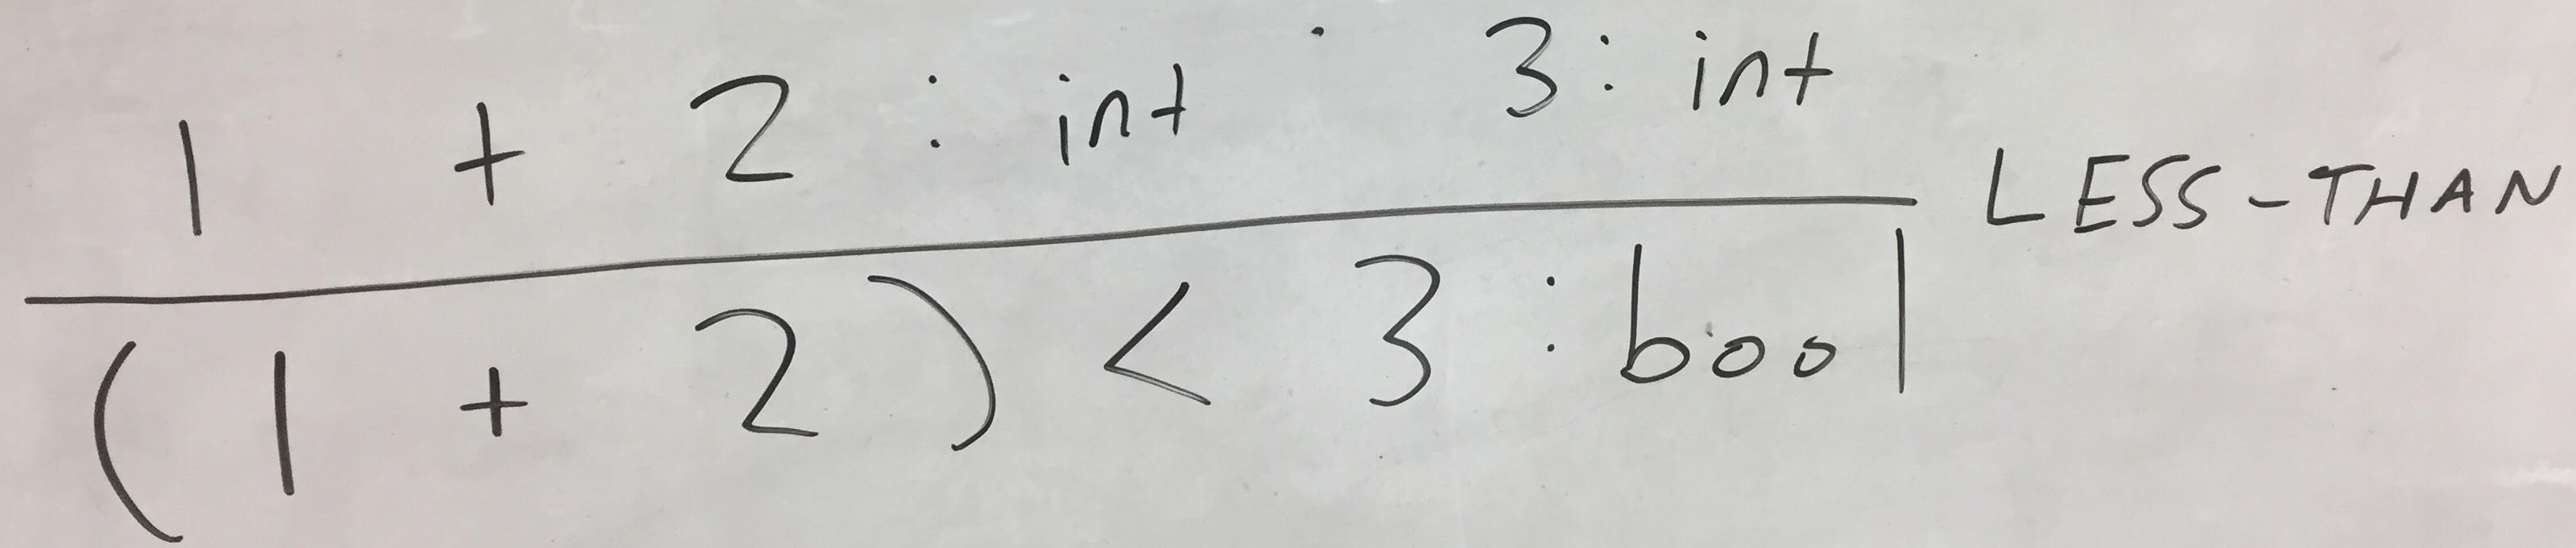
\includegraphics[width=\linewidth]{images/basic_type_proof_1.png}
\end{center}

\noindent
Note, however, we're not done: we now need to check the premises on \texttt{less-than}.
At this point, we can apply the \textsc{plus} rule to handle $1 + 2$, as shown below:

\begin{center}
  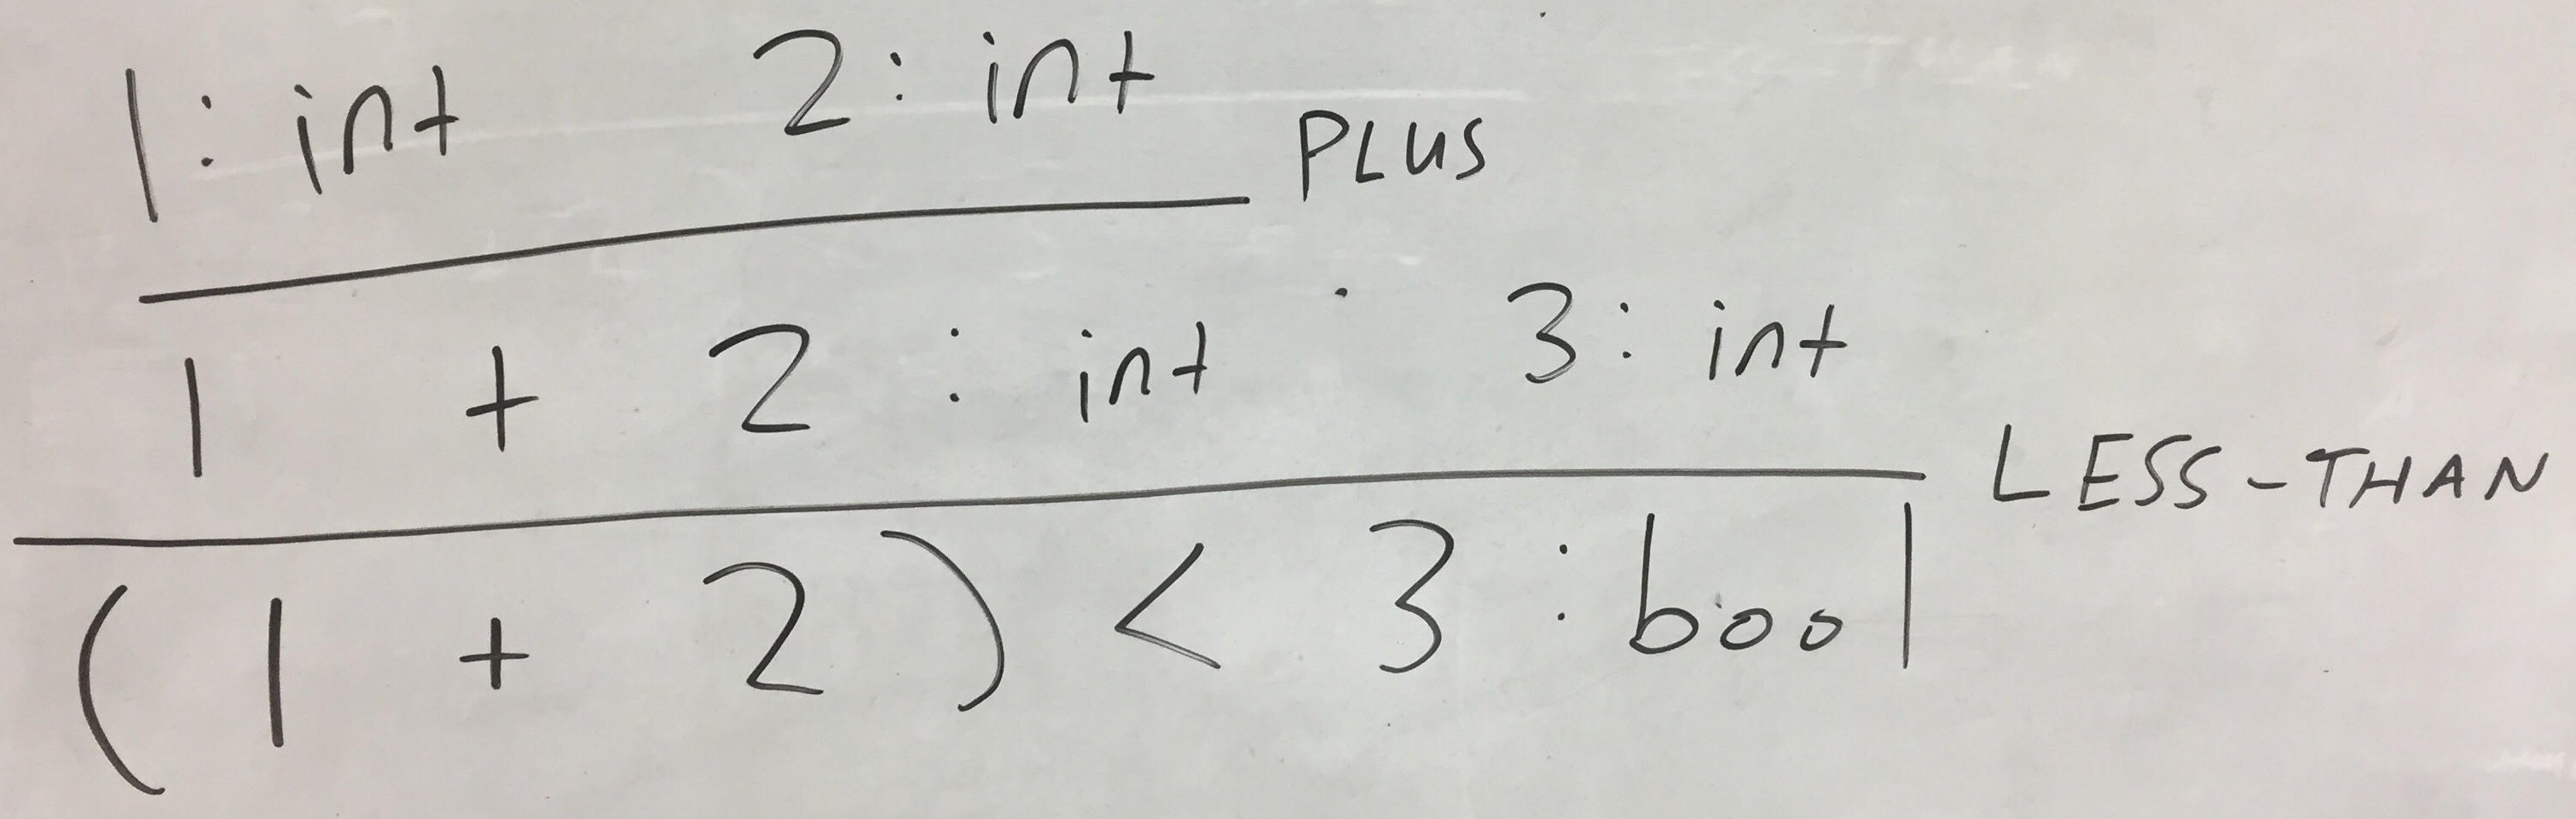
\includegraphics[width=\linewidth]{images/basic_type_proof_2.png}
\end{center}

\noindent
As for $1$, $2$, and $3$, we can handle these all with \textsc{integer}, like so:

\begin{center}
  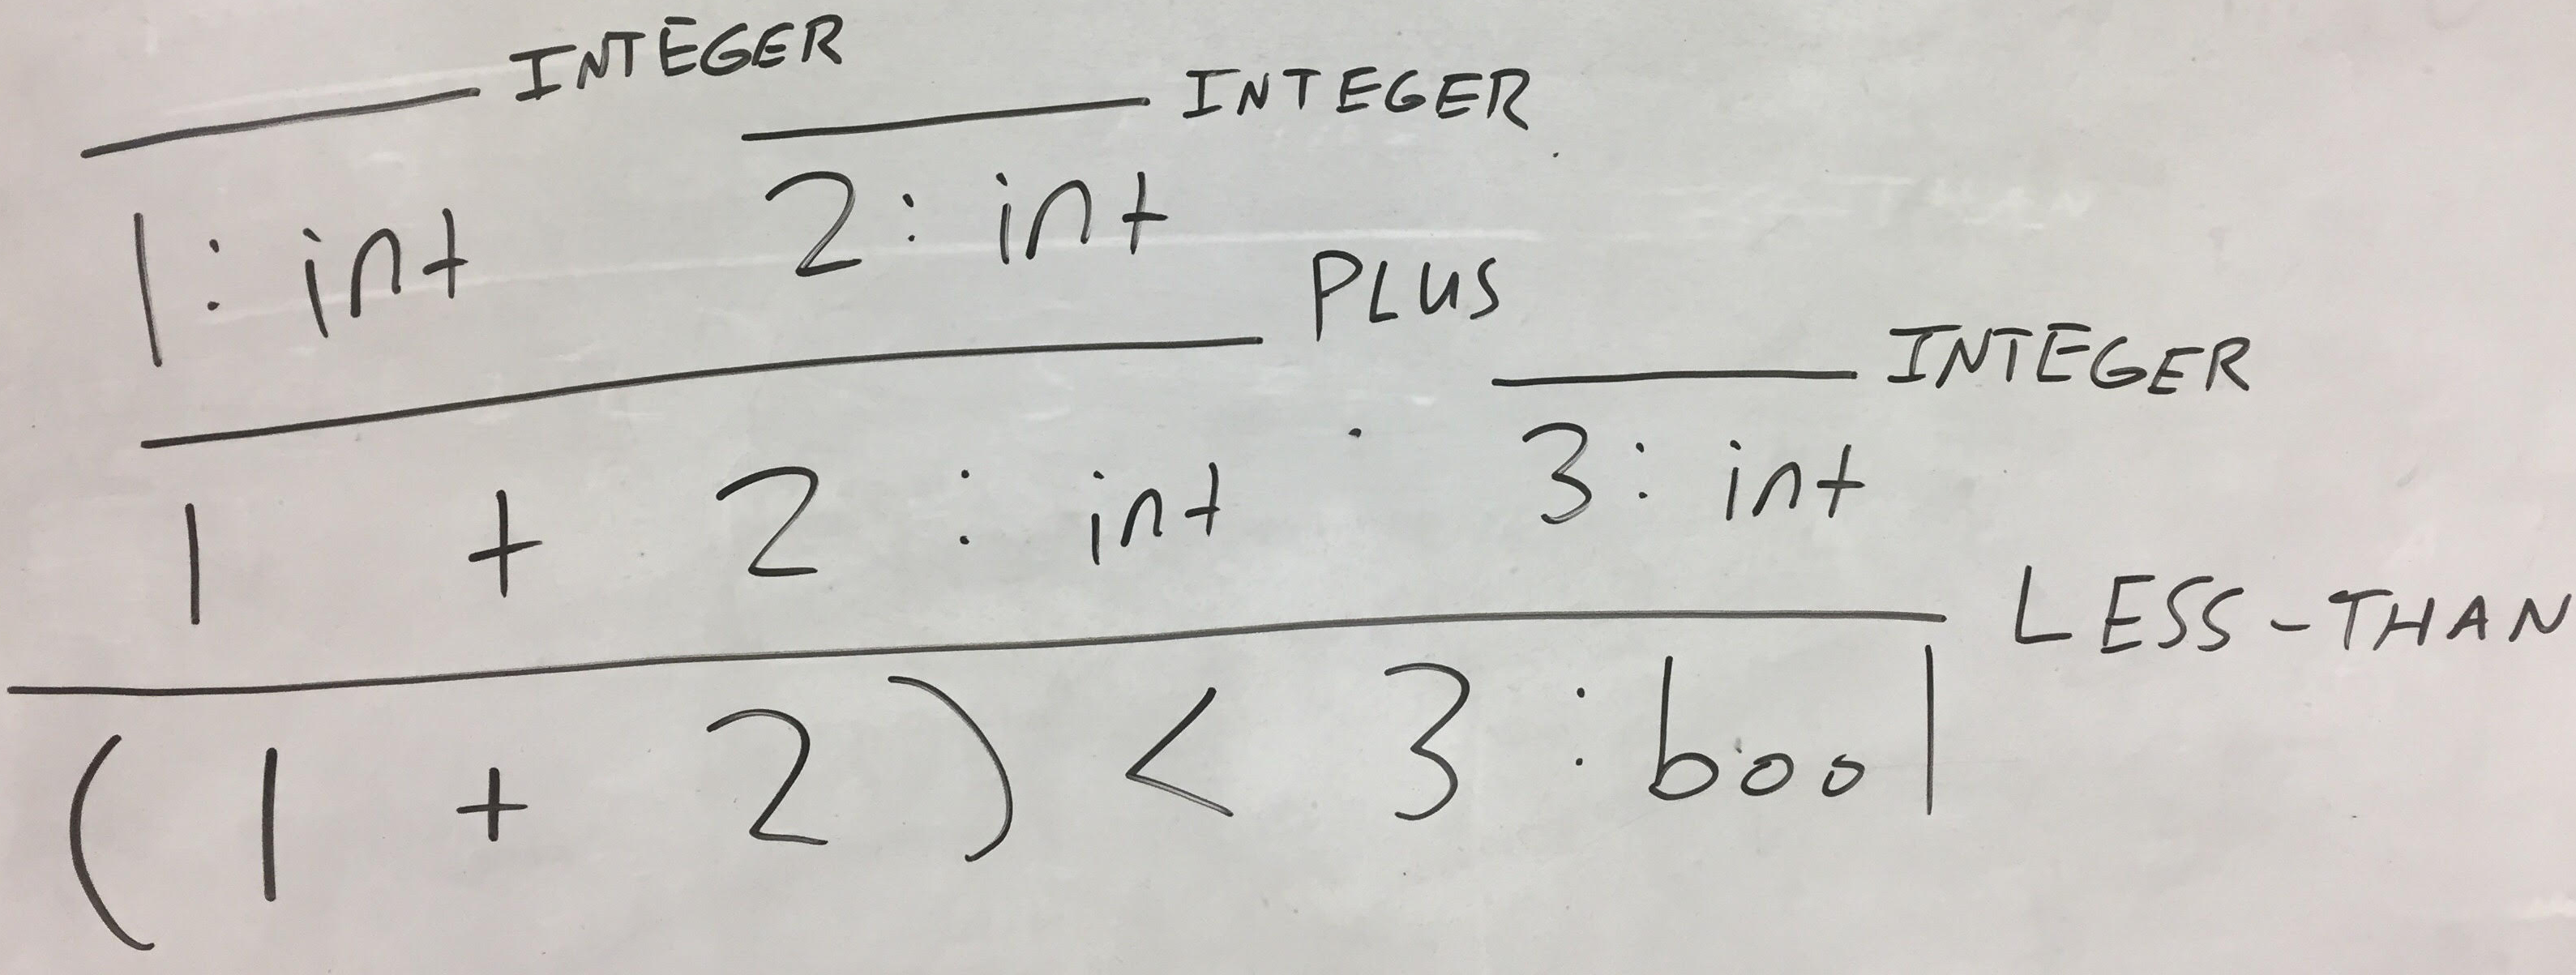
\includegraphics[width=\linewidth]{images/basic_type_proof_3.png}
\end{center}

\noindent
At this point, there is no further work to do; we have recursively checked all the necessary premises, and everything in the image starts with a line.
We now know that the type of this program is \texttt{bool}.

Sometimes, we cannot deduce the type of a program.
This usually happens because an input program is \emph{ill-typed}; that is, it has no associated type, and there is at least one type error somewhere.
To see what happens in the event of an ill-typed program, let's try to apply this same process to the following ill-typed program:

\begin{verbatim}
(1 + 2) < true
\end{verbatim}

\noindent
This starts off the same as last time, up through the application of the \textsc{integer} rule:

\begin{center}
  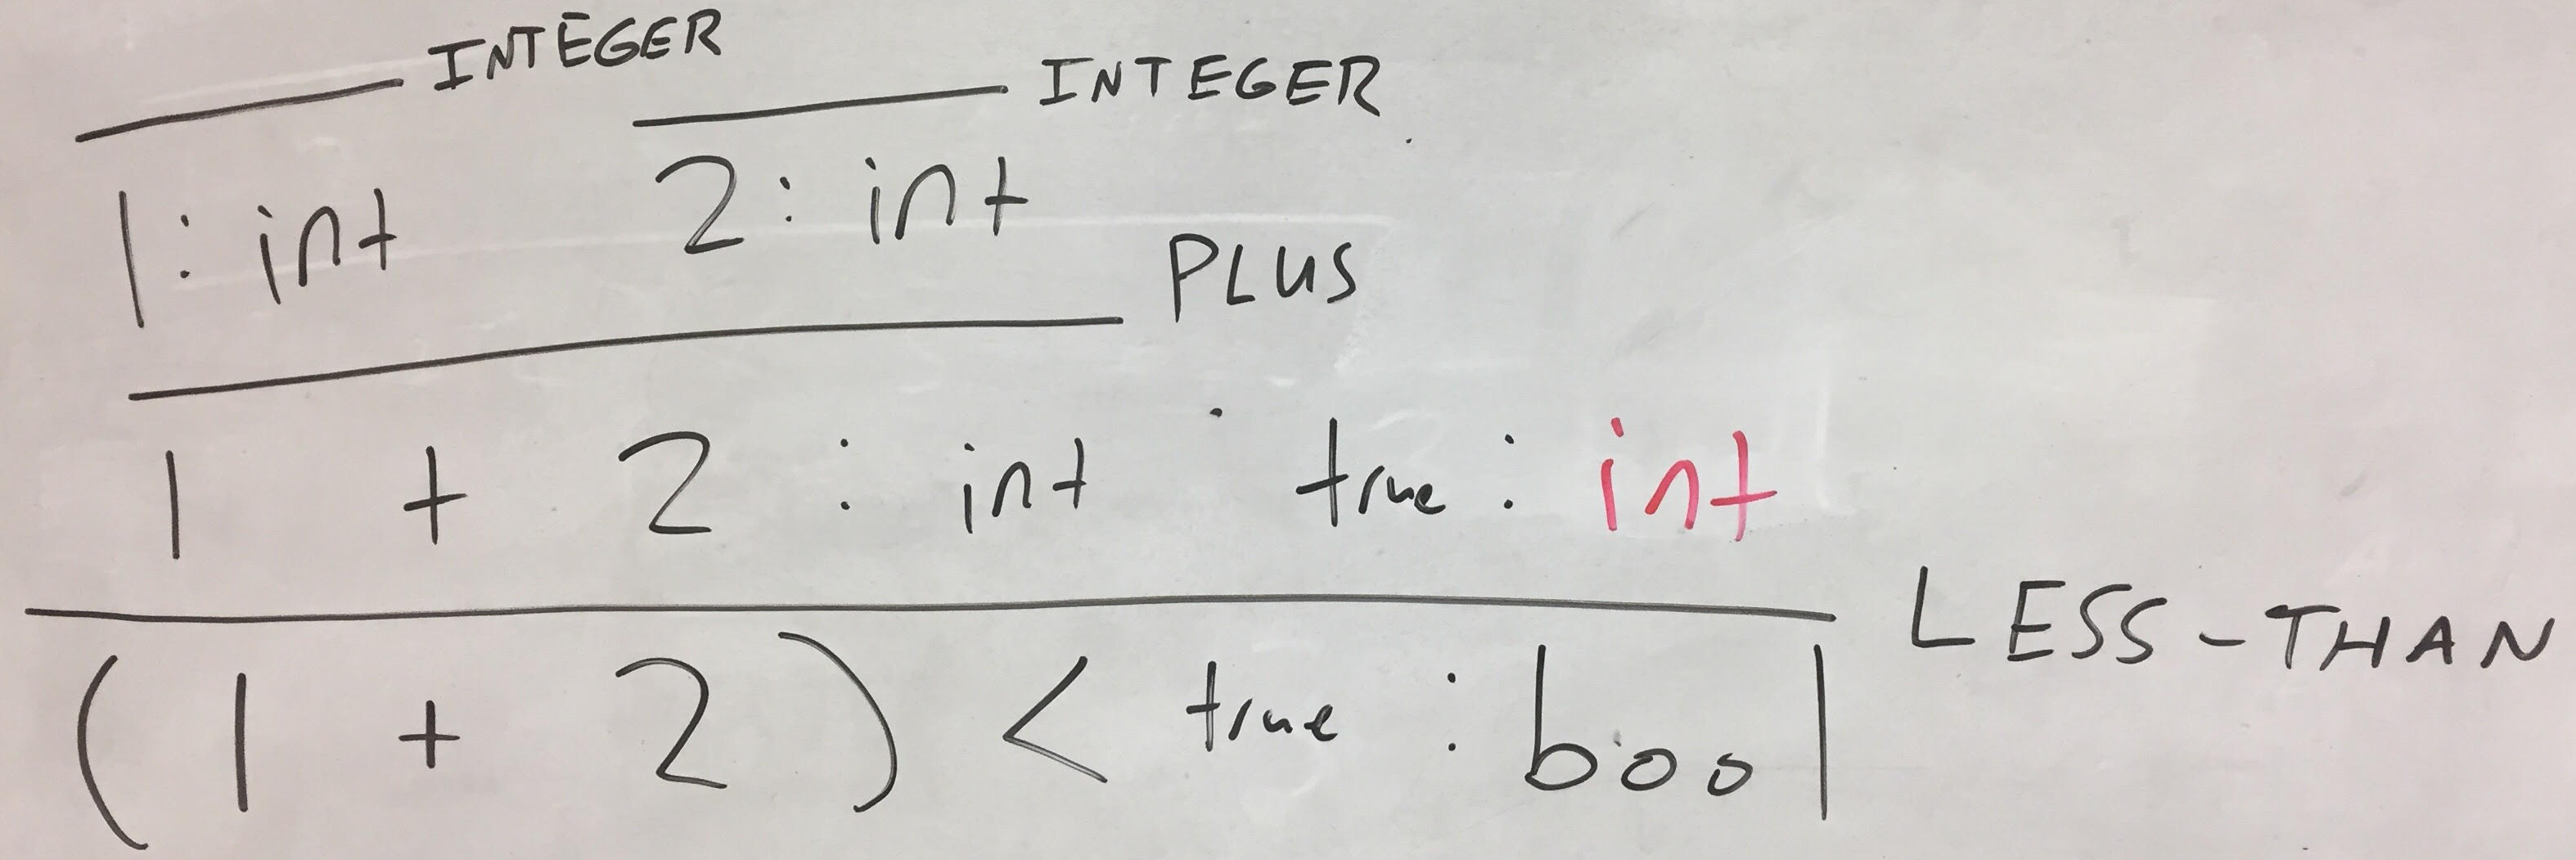
\includegraphics[width=\linewidth]{images/basic_type_error.png}
\end{center}

\noindent
However, this time around, we hit a problem, indicated by the spot in red.
The \textsc{true} rule is the only rule that directly applies to \texttt{true}, \emph{but} \textsc{true} cannot be applied here because we expect the type to be \texttt{int}, not \texttt{bool}.
That is, both the expression itself and the type need to match up with the rule, otherwise the rule cannot be applied.
Here we get stuck - we need to apply \emph{something} here (the tops of all premises need to have a line, so we're not done yet), but there is nothing we can apply.
This sort of getting stuck happens with ill-typed programs; more formally, the expression \texttt{(1 + 2) < true} has no type.

\subsubsection{Code Glimpse}
So far, the typing rules can be viewed as a way of collectively defining a Java function with the following signature:

\begin{verbatim}
public Type typeof(Exp e) throws IllTypedException
\end{verbatim}

\noindent
\ldots where:
\begin{itemize}
\item \texttt{Type} is a class representing a type
\item \texttt{Exp} is a class representing an expression
\item \texttt{IllTypedException} is an exception thrown if we discover that \texttt{e} is ill-typed.
\end{itemize}

\noindent
All the rules collectively define the implementation of \texttt{typeof}.

\subsection{Type System With Variables}
At this point, we've handled all the rules that do not involve variables.
To add variables, we'll need to keep track of which variables are in scope, along with the types of those variables.
The usual way to do this is by adding a \emph{type environment}, which maps variables in scopes to their corresponding types.
Formally, we can write this as follows:

\begin{align*}
  \Gamma \in \mtt{TypeEnv} &= \mtt{Variable} \to \mtt{Type}
\end{align*}

The above definition states that metavariable $\Gamma$ represents a mapping from $\mtt{Variable}$ to $\mtt{Type}$.
That is, if we give a $\Gamma$ a $\mtt{Variable}$, then it will give us back a $\mtt{Type}$.
That said, $\Gamma$ will only give us back a type if there is such a variable in the domain of $\Gamma$.

To make this more concrete, we will show a modified version of \texttt{typeof} as a Java signature which operates with a $\Gamma$:

\begin{verbatim}
public Type typeof(Exp e, Map<Variable, Type> gamma) throws IllTypedException
\end{verbatim}

\noindent
As shown, the type environment is literally just a plain old map data structure (or dictionary, if you prefer), where the keys are variables and the values are types.
We now pass the type environment to \texttt{typeof}, along with the expression.

There is, however, one slight distinction between $\Gamma$ and a Java map: $\Gamma$ is an \emph{immutable} map, whereas \texttt{Map} is generally \emph{mutable}.
The difference lies in what happens when we add a new key/value pair to the map.
In the math, adding a new key/value pair returns a \emph{new} map, which is the old map with the new key/value pair.
The original map is unchanged.
In contrast, in Java, adding a new key/value pair generally modifies the original map.
For what it's worth, many languages have libraries supporting the same sort of immutable data structures in code, it's just that Java doesn't have this out of the box.

Towards handling variables, we'll need to update our rules to pass along $\Gamma$.
We do this below, modifying the same rules we've seen so far:

\begin{center}
  \begin{tabular}{ccc}
    \infer[(\textsc{integer})]
      {\typeof{i}{\Gamma}{\kw{int}}}
      {}
    &
    \infer[(\textsc{true})]
      {\typeof{\kw{true}}{\Gamma}{\kw{bool}}}
      {}
    &
    \infer[(\textsc{false})]
      {\typeof{\kw{false}}{\Gamma}{\kw{bool}}}
      {}
      \\
      \\
    \infer[(\textsc{and})]
      {\typeof{e_1 \;\&\&\; e_2}{\Gamma}{\kw{bool}}}
      {\typeof{e_1}{\Gamma}{\kw{bool}} \quad \typeof{e_2}{\Gamma}{\kw{bool}}}
    &
    \infer[(\textsc{plus})]
      {\typeof{e_1 + e_2}{\Gamma}{\kw{int}}}
      {\typeof{e_1}{\Gamma}{\kw{int}} \quad \typeof{e_2}{\Gamma}{\kw{int}}}
    &
    \infer[(\textsc{less-than})]
      {\typeof{e_1 < e_2}{\Gamma}{\kw{bool}}}
      {\typeof{e_1}{\Gamma}{\kw{int}} \quad \typeof{e_2}{\Gamma}{\kw{int}}}
  \end{tabular}
\end{center}

Let's start discussion of these rules with \textsc{integer}.
The notation $\typeof{i}{\Gamma}{\kw{int}}$ says that the input type environment is $\Gamma$ and the input expression is $i$.
$\vdash$ acts as a separator of the type environment and expression inputs, just like $:$ separates the input expression from the output type.
Moving our discussion onto \textsc{and}, we can see that each recursive use of our typing rules similarly needs to have a type environment passed along as a parameter; that is, typechecking $e_1$ and $e_2$ now need $\Gamma$ as a parameter.

Note that none of these rules manipulate $\Gamma$ directly; they merely take $\Gamma$ and pass it along.
Considering our language, this should make sense; none of these rules directly involve variables, and $\Gamma$ is only needed when working with variables.
As such, we expect that these rules \emph{not} to touch $\Gamma$.

With that, let's introduce the rules that \emph{do} touch $\Gamma$, starting with variables:
\begin{center}
  \begin{tabular}{c}
    \infer[(\textsc{var})]
      {\typeof{x}{\Gamma}{\tau}}
      {x \in \texttt{dom}(\Gamma) \quad \tau = \Gamma[x]}
  \end{tabular}
\end{center}

\noindent
The notation $x \in \texttt{dom}(\Gamma)$ checks if $x$ is in the domain (\texttt{dom}) of $\Gamma$ (i.e., $x$ is contained in the type environment).
If not, the \textsc{var} rule does not apply.
The notation $\Gamma[x]$ looks up the key associated with $x$ in $\Gamma$.
The result of this lookup is bound to metavariable $\tau$.
In this context, $\tau$ is some type, and we are permitted to introduce as many metavariables as we wish.
We end up saying that the type of $x$ must be whatever $\tau$ is.

In plain English, the above rule:
\begin{itemize}
\item Checks to see if $x$ is in the type environment (in scope).
  If not, then this rule doesn't apply, and the program will be considered ill-typed.
\item Returns whatever type is associated with $x$ in $\Gamma$, performing a map lookup to check this.
\end{itemize}

From here, we introduce rules handling \texttt{let} and \texttt{assign}, shown below:

\begin{center}
  \begin{tabular}{cc}
    \infer[(\textsc{let})]
      {\typeof{\kw{let } x: \tau_1 = e_1 \kw{ in } e_2}{\Gamma}{\tau_2}}
      {\typeof{e_1}{\Gamma}{\tau_1} \quad \typeof{e_2}{\Gamma[x \mapsto \tau_1]}{\tau_2}}
    &
    \infer[(\textsc{assign})]
      {\typeof{\kw{assign } x = e_1 \kw{ in } e_2}{\Gamma}{\tau_2}}
      {x \in \texttt{dom}(\Gamma) \quad \tau_1 = \Gamma[x]\\
        \typeof{e_1}{\Gamma}{\tau_1} \quad \typeof{e_2}{\Gamma}{\tau_2}}
  \end{tabular}
\end{center}

Let's first look at \textsc{let}.
The premises of \textsc{let} say the following:
\begin{itemize}
\item $\typeof{e_1}{\Gamma}{\tau_1}$ states that $e_1$ must be of type $\tau_1$ underneath $\Gamma$.
  Notably, $\tau_1$ must be the \emph{same type} as the user annotated $x$ to be in the program.
\item The notation $\Gamma[x \mapsto \tau_1]$ adds a key/value pair to the map.
  Specifically, $x$ is the key, and $\tau_1$ is the value.
  If $x$ is already a key in $\Gamma$, then this will effectively overwrite $x$'s current value with $\tau_1$ (that is, the returned type environment will map $x$ to $\tau_1$, instead of whatever $x$ previously mapped to).
\item With the prior point in mind, $\typeof{e_2}{\Gamma[x \mapsto \tau_1]}{\tau_2}$ states to put $x$ in scope, associate it with type $\tau_1$, and determine the type of $e_2$.
  The type of $e_2$ is bound to metavariable $\tau_2$.
\item Finally, the type of a whole \texttt{let} expression is $\tau_2$, the type of $e_2$ with $x$ in scope.
\end{itemize}

Given what we know so far, \textsc{assign} should be straightforward.
This specifically states that:
\begin{itemize}
\item Whatever variable being assigned to needs to already be in scope ($x \in \texttt{dom}(\Gamma)$)
\item The type of the value we assign to $x$ ($e_1$) must be the same type as $x$ ($\tau_1 = \Gamma[x]$ and $\typeof{e_1}{\Gamma}{\tau_1}$)
\item The type of the overall assignment is whatever the type of $e_2$ is ($\tau_2$)
\end{itemize}
